\documentclass{ctexart}[UTF8]
\usepackage{dirtree}
\usepackage{listings}
\usepackage{xcolor}
\usepackage{graphicx}
\usepackage{enumerate}
\usepackage[a4paper]{geometry} 
\usepackage{amsmath,amsthm,mathtools,amssymb}
\usepackage{mathtools}
\usepackage{diagbox}
\usepackage{multirow,makecell}
\usepackage{float}
\usepackage{url}
\usepackage[nottoc]{tocbibind}
\usepackage{float}
\newcommand{\refe}[1]{Eq.\ref{#1}}
\newcommand{\reft}[1]{Theory.\ref{#1}\ }
\newcommand{\reff}[1]{图\ref{#1}\ }
\lstset{
 columns=fixed,
 numbers=left,                                        % 在左侧显示行号
 numberstyle=\tiny\color{gray},                       % 设定行号格式
 basicstyle=\small\ttfamily,
 frame=none,                                          % 不显示背景边框
 backgroundcolor=\color[RGB]{245,245,244},            % 设定背景颜色
 keywordstyle=\color[RGB]{40,40,255},                 % 设定关键字颜色
 numberstyle=\footnotesize\color{darkgray},           
 commentstyle=\color{gray}\ttfamily,                  % 设置代码注释的格式
 stringstyle=\rmfamily\slshape\color[RGB]{128,0,0},   % 设置字符串格式
 showstringspaces=false,
 breaklines=true,
 language=c++
}
\newtheorem{theorem}{Theory}[section]
\geometry{bottom=2cm,left=1cm,right=1cm}
\title{上机10}
\author{张配天-2018202180}
\begin{document}
    \maketitle
    \tableofcontents
    \clearpage
    \section{霍夫曼编码}
    \subsection{问题描述}
    求解霍夫曼编码。
    \subsubsection{输入}
    字母表,其中每个字母对应一个频率。
    \subsubsection{输出}
    字母表,每个字母对应其霍夫曼编码。
    \subsection{算法思路}
    \subsubsection{贪心策略}
    每次选择出现频率最小的两个节点,将两者并为一个新节点的左右孩子,新节点的频率为两者频率之和,直到所有节点都已经称为叶子。
    \subsubsection{贪心选择性质}
    \begin{theorem}
        \underline{贪心选择性}即证明:对于字母表中出现频率最小的两个字母,可以将其合并到霍夫曼树的一个节点中得到最优前缀码;即两者的最优前缀码仅有最后一位不同。
    \end{theorem}
    \textbf{证明:}设最优前缀码树T中频率最小的两个节点分别为$x$,$y$,考虑树中不同于$x,y$的任意两个顶点$a,b$,分别交换$a,x$和$b,y$,得到新树$T',T''$,
    根据代价公式有\begin{align*}
        B(T) - B(T') &= \sum_{c\in T}freq(c) \cdot d(c) - \sum_{c'\in T'}freq(c') \cdot d(c')\\
                    &= (freq(x) - freq(a))\cdot d(x) + (freq(a) - freq(x))\cdot d(a)\\
                    &= (d(x) - d(a))\cdot (freq(x) - freq(a)) \\
                    &< 0
    \end{align*}
    同理可证将$y$与$b$交换得到的新树$T''$的代价高于$T$,因此$T$为最优前缀码树,得证。
    \subsubsection{最优子结构性质}
    \begin{theorem}
        \underline{最优子结构性}即证明:对于一颗最优前缀编码树,如果去掉其中频率最低的两个节点,引入一个新的节点,该新节点的频率是去掉的两个节点的频率之和,且两个去掉的节点是该新节点的叶子,那么新形成的树也是一个最优前缀编码树。
    \end{theorem}
    \textbf{证明:}考虑最优前缀编码树$T$,其中出现频率最低的两个节点分别为$x,y$,将两者并为一个新节点记作$z$,形成的树记作$T'$,则
    \begin{equation}
        B(T') = B(T) + freq(x)\cdot d(x) + freq(y) \cdot d(y)
    \end{equation}
    于是,假设得到的$T'$不是一个最优前缀编码树,那么存在最优前缀编码树$T''$包含兄弟节点$x,y$,且$B(T'') < B(T')$,于是将$T''$中的$x,y$子树替换为$x,y$,得到$T'''$,那么有$B(T''') < B(T)$与假设矛盾,因此得证。
    \subsection{复杂度分析}
    设字母表长度为$n$,那么有\begin{itemize}
        \item 第40-45行维护堆,涉及到两次pop和一次push,每一次操作有$O(lgn)$,因此有时间复杂度$O(lgn)$
        \item 第39行一个大循环,有时间复杂度$O(n)$
        \item 回溯算法55-73行,只会输出$n$个字母的前缀码,而每次栈操作复杂度O(1),因此总时间复杂度$O(n)$
    \end{itemize}
    \par 因此,总时间复杂度$O(nlogn)$。
    \subsection{源码}
    \lstinputlisting[language=c++]{d:/repositories/Algorithm/Instances/Huffman.cpp}    
    \subsection{运行截图}
    \begin{figure}[H]
        \centering
        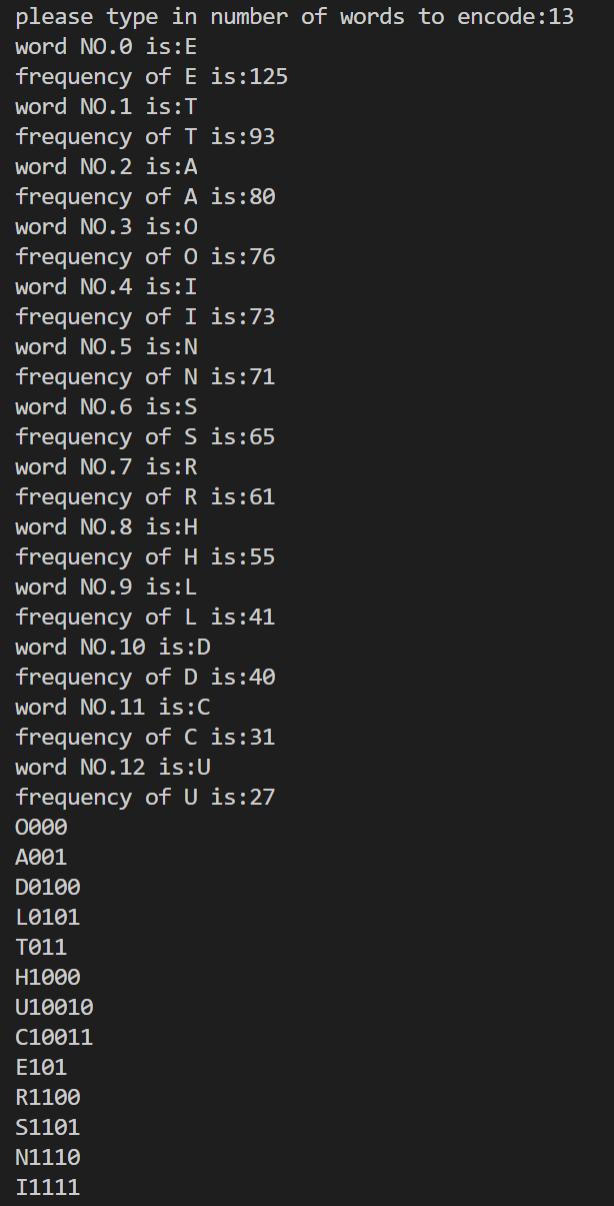
\includegraphics[width=8cm,height=16cm]{resources/10_1.png}
    \end{figure}
    
    \section{迪杰特斯拉算法}
    \subsection{问题描述}
    迪杰特斯拉算法求最短源路径。
    \subsubsection{输入}
    有向图的领结矩阵,$i,j$元为对应弧的权重;源顶点$start$。
    \subsubsection{输出}
    源顶点到其余各个定点的最短路径长度,以及到特定节点的路径。
    \subsection{算法思路}
    \subsubsection{贪心策略}
    从$V-S$中选择具有最短特殊路径的顶点$u$,确定从源到$u$的最短路径。
    \subsubsection{贪心选择性质}
    \begin{theorem}
        \underline{贪心选择性}即证明:每次选择最短的特殊路径,最终构成的源路径最短。
    \end{theorem}
    \textbf{证明:}假设存在一条更短的路,之后徘徊于$S$内外若干次,最后到达$u$,首先根据贪心策略,有源到$x$的距离$dist(v,x) \le dist[x]$;
    又根据假设有$dist(v,x) + dist(x,u) = dist(v,u) < dist[u]$,因为$dist(x,u) > 0$,于是有$dist[u] > dist[x]$,矛盾,得证。
    \subsubsection{最优子结构性质}
    \begin{theorem}
        \underline{最优子结构性}即证明:对于源路径$start\rightarrow end$,如果删去最后一段路径,那么$start\rightarrow end'$仍然是最短源路径。 
    \end{theorem}
    \textbf{证明:}使用剪贴法,如果新得到的路径$l'$即$start\rightarrow end'$不是最短路径,那么有从$start\rightarrow end'$的最短路径$l''$,将$l$中的$l'$替换为$l''$则得到$l'''$且路径长度小于$l$,矛盾。
    \subsection{复杂度分析}
    设有向图一共有$n$个顶点,则有 \begin{itemize}
        \item 39-41行,46-49行均为$O(n)$的循环
        \item 37行外层循环$n$次
        \item 回溯算法中60-62行最多入栈$n-1$个顶点,其余操作时间复杂度均为$O(1)$,因此回溯\textbf{到给定顶点路径的}时间复杂度为$O(n)$
    \end{itemize}
    \par 因此,总时间复杂度$O(n^2)$。
    \subsection{源码}
    \lstinputlisting[language=python]{D:/repositories/Algorithm/Instances/Djikstra.py}
    \subsection{运行截图}
    \begin{figure}[H]
        \centering
        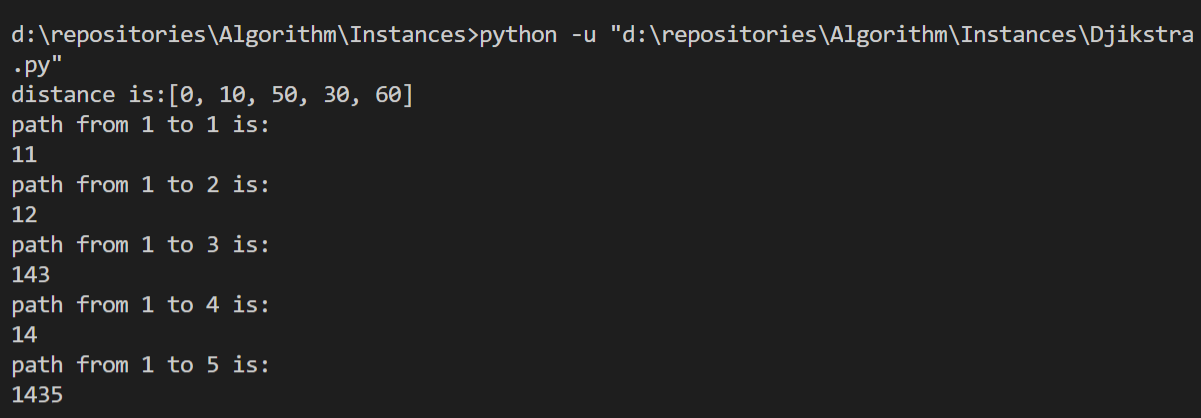
\includegraphics[width=14cm]{resources/10_2.png}
    \end{figure}
\end{document}

